\documentclass[10pt,a4paper]{article}
\usepackage[italian]{babel}
% Use Helvetica
\usepackage[scaled]{helvet}
% Use it as default
\renewcommand\familydefault{\sfdefault}
\usepackage[T1]{fontenc}\usepackage[utf8]{inputenc}

\usepackage{enumitem}
\setlist[itemize]{noitemsep, leftmargin=*}
\usepackage{amsmath}
\usepackage{graphicx}
\usepackage{tabularx}
\usepackage{caption}
\usepackage{ragged2e}
\usepackage{fancyhdr}
\captionsetup[figure]{labelformat=empty}
\usepackage{multicol}
\setlength\columnsep{30pt}
%\setlength{\columnseprule}{0.4pt}
% Add margins
\usepackage{geometry}
\geometry{
  a4paper,
  left=1.4cm,
  right=1.4cm,
  headheight=12pt,
  top=2.5cm,
  bottom=1.5cm,
  footskip=0cm
}
% Header page numbering
\pagestyle{fancy}
\fancyhf{}
\renewcommand{\headrulewidth}{0pt}
\fancyhead[R]{\thepage}

% Images
\graphicspath{ {./images/} }

% Code
\newcommand{\code}{\texttt}
\usepackage{listings}
\lstset{
    basicstyle=\ttfamily,
    mathescape=true,
    resetmargins=true}
% Lists have tiny bullet
\renewcommand\labelitemi{\textendash}
\renewcommand\labelitemii{\textendash}
\renewcommand\labelitemiii{\textendash}

\author{Andrea Franchini}
\title{Appunti di Algoritmi}

\begin{document}
\section*{Complessit\`a del calcolo}
   \subsection*{Caso pessimo}
   $T_M(n) = \max\left\{T_M(x), |x|=n\right\}$\\
   $S_M(n) = \max\left\{T_M(x), |x|=n\right\}$
   \subsection*{Notazioni}
   \begin{itemize}
       \item O-grande: limite asintotico superiore.\\
       Data $g(n)$, $O(g(n)) = \left\{f(n) \mid \exists c,n_0 \left(c,n_0 > 0 : \forall n \ge n_0 0 \le f(n) \le cg(n)\right)\right\}$

       \item $\Omega$-grande: limite asintotico inferiore.\\
       Data $g(n)$, $\Omega(g(n)) = \left\{f(n) \mid \exists c,n_0 \left(c,n_0 > 0 : \forall n \ge n_0 0 \le cg(n)  \le f(n) \right)\right\}$

       \item $\Theta$-grande: limite asintotico sia superiore sia inferiore.\\
       Data $g(n)$, $\Theta(g(n)) = \left\{f(n) \mid \exists c_1,c_2,n_0 \left(c_1,c_2,n_0 > 0 : \forall n \ge n_0 0 \le c_1g(n) \le f(n) \le c_2g(n)\right)\right\}$
   \end{itemize}
\section*{Teoremi di accelererazione lineare}
\begin{itemize}
    \item Se $L$ \`e accettato da una MT $M$ a $k$ nastri con complessit\`a $S_M(n)$, per ogni $c > 0 (c \in R)$ si pu\`o costruire una MT $M'$ a $k$ nastri con complessit\`a $S_{M'}(n) < c S_M(n)$
    
    \item Se $L$ \`e accettato da una MT $M$ a $k$ nastri con complessit\`a $S_M(n)$, si pu\`o costruire una MT $M'$ a 1 nastro (\textit{non} a nastro singolo) con complessit\`a $S_{M'}(n) = S_M(n)$

    \item Se $L$ \`e accettato da una MT $M$ a $k$ nastri con complessit\`a $S_M(n)$, per ogni $c > 0 (c \in R)$ si pu\`o costruire una MT $M'$ a 1 nastro con complessit\`a $S_{M'}(n) < cS_M(n)$

    \item Se $L$ \`e accettato da una MT $M$ a $k$ nastri con complessit\`a $T_M(n)$, per ogni $c > 0 (c \in R)$ si pu\`o costruire una MT $M'$ (a $k+1$ nastri) con complessit\`a $T_{M'}(n) = \max \left\{n+1, cT_M(n)\right\}$
\end{itemize}
\paragraph{Conseguenze pratiche}
\begin{itemize}
    \item Lo schema di dimostrazione \`e valido per qualsiasi tipo di modello di calcolo, quindi anche per calcolatori reali (es.: aumentare il parallelismo fisico (16bit $\rightarrow$ 32bit $\rightarrow \dots$)).
    \item Aumentando la potenza di calcolo in termini di risorse disponibili si pu\`o aumentare la velocit\`a di esecuzione, ma il miglioramento \`e al pi\`u lineare.
    \item Miglioramenti di grandezza superiore possono essere ottenuti solo cambiando algoritmo e non in modo automatico.
\end{itemize}

\section*{Macchina RAM}
\begin{multicols}{2}
\subsection*{Glossario}
\begin{itemize}
    \item\textit{Accumulatore}: \`e la prima cella del modello della memoria, indicata con \code{M[0]}.
    \item\textit{Immediato}: \`e un numero intero.
    \item\textit{ADD}: Sono le operazioni elementari di somma (\code{ADD}), sottrazione (\code{SUB}), moltiplicazione (\code{MULT}), divisione (\code{DIV}).
\end{itemize}
\subsection*{Costi Logaritmici}
Il costo della copia di un numero $n$ da una cella all'altra \`e tante micro-operazioni elementari quanti sono i bit necessari a codificare $n$, cio\`e $\log(n)$.\\
Il costo dell'accesso ad una cella di posizione $n$-esima \`e l'apertura di $\log(n)$ gate logici ad altrettanti banchi di memoria.\\
In forma sintetica:
\begin{equation*}
    l(i) = \textit{if } i=0 \textit{ then } 1
    \textit{ else } \left\lfloor\log_2|i|\right\rfloor + 1
\end{equation*}

\subsection*{Teorema di correlazione polinomiale}
Sotto ``ragionevoli'' ipotesi di criteri di costo (il criterio di costo costante per la RAM non \`e ragionevole) se un problema \`e risolvibile mediante un modello di calcolo $M_1$ con complessit\`a $C_1(n)$, allora \`e risolvibile da qualsiasi altro modello di calcolo $M_2$ con complessit\`a $C_2(n) \le P_2(C_1(n))$, essendo $P_2$ un opportuno polinomio.
\end{multicols}

\hspace*{-0.7cm}
\begin{tabularx}{\linewidth}{l r|l|l|X}
    \hline
    Comando && Operazione & Complessit\`a & Descrizione\\
    \hline
    \code{LOAD} &\code{X}& \code{M[0] = M[X]} & $l(x)$ & Carica in \code{M[0]} il contenuto della cella X\\
    \code{LOAD=} &\code{X}& \code{M[0] = X} & $l(x) + l(M[x])$ & Carica in \code{M[0]} l'immediato X\\
    \code{LOAD*} &\code{X}& \code{M[0] = M[M[X]]} & $l(x) + l(M[x]) + l(M[M[x]])$ & Carica in \code{M[0]} dall'indirizzo M[X]\\
    \code{STORE} &\code{X}& \code{M[X] = M[0]} & $l(x) + l(M[0])$ & Carica in \code{M[X]} il contenuto di M[0]\\
    \code{STORE*} &\code{X}& \code{M[X] = M[M[0]]} & $l(x) + l(M[x]) + l(M[0])$& Carica in \code{M[X]} dall'indirizzo M[0]\\
    \code{ADD} &\code{X}& \code{M[0] = M[0] + M[X]} & $l(M[0]) + l(x) + l(M[x])$ & Carica in \code{M[0]} il risultato dell'operazione\\
    \code{ADD=} &\code{X}& \code{M[0] = M[0] + X} & $l(M[0]) + l(x)$ &\\
    \code{ADD*} &\code{X}& \code{M[0] = M[0] + M[M[X]]} & $l(M[0]) + l(x) + l(M[x]) + l(M[M[x]])$ &\\

    \code{READ} &\code{X}& \code{M[X] = read()} & $l(\textit{input value}) + l(x)$& Salva in X il valore letto in input\\
    \code{READ*} &\code{X}& & $l(\textit{input value}) + l(x) + l(M[x])$ & \\
    \code{WRITE} &\code{X}& write(M[X] ) & $l(x) + l(M[x])$ & Scrive in output il valore di X\\
    \code{WRITE=} &\code{X}& write(X) & $l(x)$ & Scrive in output l'immediato X\\
    \code{WRITE*} &\code{X}& write(M[M[X]]) & $l(x) + l(M[x]) + l(M[M[x]])$ & Scrive in output l'indirizzo di X\\
    \code{JUMP} &\code{label}& \code{PC= b(label)} & $1$ & Salta alla label indicata\\
    \code{JZ} &\code{label}& \code{if M[0] == 0}& $l(M[0])$& Salta alla label indicata se l'accumulatore \`e $0$.\\
    \code{JGZ} &\code{label}& \code{if M[0] > 0}& $l(M[0])$& Salta alla label indicata se l'accumulatore \`e maggiore di $0$.\\
    \code{HALT} && & $1$& Interrompe l'esecuzione del programma.\\
\end{tabularx}

\section*{Algoritmi}

Si adotta il criterio di \textbf{costo costante} (manipoliamo numeri che non richiedono quantit\`a di memoria molto pi\`u grandi della dimensione dell'input). \\
Ogni istruzione viene eseguita in un tempo costante $c_i$.

\subsection*{Complessit\`a di un algoritmo \textit{divide et impera}}
\begin{itemize}
    \item Si divide il problem in $b$ sottoproblemi, ciascuno con dimensione $\frac{1}{b}$.
    \item Se il problema ha dimensione $n$ piccola a sufficienza ($n < c$, $c$ costante caratteristica del problema), esso pu\`o essere risolto in tempo costante ($\Theta(1)$).
    \item $D(n)$ \`e il costo di dividere il problema, e $C(n)$ \`e il costo di ricombinare i sottoproblemi. $T(n)$ \`e il costo per risolvere il problema totale.
\end{itemize}
\begin{equation*}
    \text{Equazione di Ricorrenza} \quad T(n) = 
    \begin{cases}
        \Theta(1) \qquad \text{se } n < c\\
        D(n) + aT(\frac{n}{b}) + C(n) \quad  \text{altrimenti}
    \end{cases}
\end{equation*}

\pagebreak

\begin{multicols*}{2}
\subsection*{Insertion Sort}
\begin{lstlisting}
INSERTION-SORT(A)
    for j = 2 to A.length
        key = A[j]
    i = j - 1
    while i > 0 and A[i] > key
        A[i+1] = A[i]
        i = i - 1
    A[i+1] = key
\end{lstlisting}
\subsection*{Merge Sort}
\begin{lstlisting}
MERGE-SORT(A, p, r)
    if p < r
        q = $\lfloor$(p+r)/2$\rfloor$
        MERGE-SORT(A, p, q)
        MERGE-SORT(A, q+1, r)
        MERGE(A, p, q, r)

MERGE (A, p, q, r)
$n_1$ = q-p+1
$n_2$ = r-q
CreaArray(L[1...$n_1$+1] e R[1...$n_2$+1])
for i = 1 to $n_1$
    L[i] = A[p+i-1]
for j = 1 to $n_2$
    R[j] = A[q+j]
L[$n_1$+1] = $\infty$
R[$n_2$+1] = $\infty$
i = 1
j = 2
for k = p to r
    if L[i] <= R[j]
        A[k] = L[i]
        i = i+1
    else
        A[k] = R[j]
        j = j+1
\end{lstlisting}
\subsection*{Heapsort}
\begin{lstlisting}
PARENT(i)
    return $\lfloor i/2\rfloor$
LEFT(i)
    return 2*i
RIGHT(i)
    return 2*i+1

MAX-HEAPIFY(A, i)
    l = LEFT(i)
    r = RIGHT(i)
    if l <= A.heapsize and A[l] > A[i]
        max = l
    else
        max = i
    if r <= A.heapsize
    and A[r] > A[max]
        max = r
    if max != i
        swap A[i] $\leftrightarrow$ A[max]
        MAX-HEAPIFY(A, max)

BUILD-MAX-HEAP(A)
    A.heapsize = A.length
    for i = A.length/2 to 1
        MAX-HEAPIFY(A, i)

HEAPSORT(A)
    BUILD-MAX-HEAP(A)
    for i = A.length to 2
        swap A[1] $\leftrightarrow$ A[i]
        A.heapsize = A.heapsize - 1
        MAX-HEAPIFY(A, 1)
\end{lstlisting}
\subsection*{Quicksort}
\begin{lstlisting}
QUICKSORT(A, p, r)
    if p < r
        q = PARTITION(A, p, r)
        QUICKSORT(A, p, q-1)
        QUICKSORT(A, q+1, r)

PARTITION(A, p, r)
    x = A[r]
    i = p-1
    for j = p to r-1
        if A[j] <= X
            i = i+1
            swap A[i] $\leftrightarrow$ A[j]
    swap A[i+1] $\leftrightarrow$ A[r]
    return i+1
\end{lstlisting}
\subsection*{Counting Sort}
\begin{lstlisting}
COUNTING-SORT(A, B, k)
    for i = 0 to k
        C[i] = 0
    for j = 1 to A.length
        C[A[j]] = C[A[j]] + 1
    for i = 1 to k
        C[i] = C[i] + C[i-1]
    for j = A.length to 1
        B[C[A[j]]] = A[j]
        C[A[j]] = C[A[j]] - 1
\end{lstlisting}
\end{multicols*}

\pagebreak

\subsection*{Risoluzione di ricorrenze}
\begin{itemize}
    \item Metodo della sostituzione \begin{itemize}
        \item formulare un'ipotesi di soluzione
        \item sostituire la soluzione nella ricorrenza, e dimostrazione (per induzione) che \`e in effetti una soluzione
    \end{itemize}
    \item Teorema dell'esperto (Master Theorem) \begin{itemize}
        \item Data la ricorrenza $T(n) = aT(\frac{n}{b}) + f(n)$, in cui $a\ge1$, $b>1$, $\left\lfloor\frac{n}{b}\right\rfloor$ o $\left\lceil\frac{n}{b}\right\rceil$.
        \begin{enumerate}
            \item se $f(n) = O\left(n^{\log_ba-\varepsilon}\right)$ per qualche $\varepsilon>0$, allora $T(n)=\varTheta\left(n^{\log_ba}\right)$
            \item se $f(n) = \varTheta\left(n^{\log_ba}\right)$, allora $T(n)=\varTheta\left(n^{\log_ba}\log(n)\right)$
            \item se $f(n) = \varOmega\left(n^{\log_ba+\varepsilon}\right)$ per qualche $\varepsilon>0$, e $af\left(\frac{n}{b}\right)\le cf(n)$ per qualche $c<1$ e per tutti gli $n$ grandi a sufficienza, allora $T(n)=\varTheta(f(n))$
        \end{enumerate}
        \item Se $f(n) = \varTheta\left(n^k\right)$, con $k$ una qualche costante:
        \begin{enumerate}
            \item se $k < \log_ba \rightarrow T(n) = \varTheta\left(n^{\log_ba}\right)$
            \item se $k = \log_ba \rightarrow T(n) = \varTheta\left(n^k\log(n)\right)$
            \item se $k > \log_ba \rightarrow T(n) = \varTheta\left(n^k\right)$
        \end{enumerate}
    \end{itemize}
\end{itemize}

\section*{Strutture dati}

\begin{multicols*}{2}
\code{S} = collezione, \code{k} = chiave
\subsection*{Operazioni comuni}
\begin{itemize}
    \item \code{SEARCH(S, k)}
    \item \code{INSERT(S, k)}
    \item \code{DELETE(S, k)}
    \item \code{MINIMUM(S)}
    \item \code{MAXIMUM(S)}
    \item \code{SUCCESSOR(S, k)}
    \item \code{PREDECESSOR(S, k)}
\end{itemize}
\subsection*{Pila/Stack}
\begin{itemize}
    \item Politica \textbf{LIFO} (Last In First Out)
    \item \code{POP(S)} cancella l'elemento in cima alla pila e lo restituisce
    \item \code{PUSH(S)} aggiunge un elemento in cima alla pila
    \item \code{S.top} è l'elemento in cima alla pila
    \item Se può contenere al massimo $n$ elementi, si implementa come un array di dimensione $n$
\end{itemize}
\subsection*{Code/Queue}
\begin{itemize}
    \item Politica \textbf{FIFO} (First In First Out)
    \item \code{ENQUEUE(S)} inserisce un elemento in fondo alla coda
    \item \code{DEQUEUE(S)} cancella il primo elemento dalla coda
    \item \code{S.head} è l'elemento nella coda da più tempo
    \item \code{S.tail} è la posizione dove verrà inserito il nuovo elemento
\end{itemize}
\subsection*{Lista doppiamente concatenata}
\begin{itemize}
    \item Ogni oggetto $x$ della lista $L$ è costituito da 3 attributi:
    \begin{itemize}
        \item \code{key} è il contenuto
        \item \code{next} è il puntatore all'oggetto seguente
        \item \code{prev} è il puntatore all'oggetto precedente
    \end{itemize}
    \item Se \code{x.next == nil}, \code{x} non ha successore
    \item Se \code{x.prev == nil}, \code{x} non ha predecessore
    \item \code{L.head} è il puntatore al primo elemento della lista
\end{itemize}
\subsubsection*{Costi di una lista}
\begin{tabular}{l l}
    Search & $T(n) = O(n)$\\
    Insert & $T(n) = O(1)$\\
    Delete & $T(n) = O(1)$\\
\end{tabular}
\subsection*{Dizionario/Dictionary}
\begin{itemize}
    \item Supporta solo le operazioni di \code{INSERT}, \code{DELETE}, \code{SEARCH}
    \item Agli oggetti di un dizionario si accede tramite le chiavi, che sono numeri interi
    \item Se la cardinalità $m$ dell'insieme delle possibili chiavi è piccola, conviene l'indirizzamento diretto, cioè un array di dimensione $m$ dove ogni chiave $k$ è mappata alla cella corrispondente
\end{itemize}
\subsubsection*{Costi di un dizionario}
\begin{tabular}{l l}
    Search & $T(n) = O(1)$\\
    Insert & $T(n) = O(1)$\\
    Delete & $T(n) = O(1)$\\
\end{tabular}
\subsection*{Tabella Hash/Hash Table}
\begin{itemize}
    \item Ho una funzione hash $h(k) \in N$ che converte una chiave di qualsiasi tipo in un intero tra $0$ e $m$
    \item Se la dimensione $m$ della mia tabella è tale che $m \ll |U|$, ci sono sicuramente chiavi tali che $h(k_1) = h(k_2)$: in questo caso ho delle collisioni.
\end{itemize}
\subsubsection*{Concatenamento}
\begin{itemize}
    \item \emph{Idea:} gli oggetti che vengono mappati sullo stesso slot vengono messi in una lista $L$ concatenata, di lunghezza $|M|L| = [h(k)]|$
\end{itemize}
\begin{tabular}{l l l}
    Search & $T(n) = |M[h(k)]|$ & $M$ è la hash table\\
    Insert & $T(n) = O(1)$ & $x \not\in M$\\
    Delete (1) & $T(n) = O(1)$ & double-linked $L$\\
    Delete (2) & $T(n) = |M[h(k)]|$ & single-linked $L$\\
\end{tabular}
\begin{itemize}
    \item Nel caso pessimo si ha la complessità di una ricerca in una lista di $n$ elementi, cioè $T(n) = O(n)$.
    \item $\alpha = \frac{n}{m}$ è il \emph{fattore di carico}
    \item $0\le n \le |U| \rightarrow 0 \le \alpha \le \frac{|U|}{m}$
\end{itemize}
\subsubsection*{Ipotesi di hashing uniforme semplice}
\begin{itemize}
    \item Ogni chiave ha la stessa probabilità $\frac{1}{m}$ di finire in una qualsiasi delle $m$ celle di $T$, indipendentemente dalle chiavi inserite. La lunghezza media di una lista è quindi:
    \begin{equation*}
        E\left(n_j\right) = \frac{1}{m}\sum^m_{i=1}n_i = \frac{n}{m} = \alpha
    \end{equation*}
    \item Il tempo medio per cercare una chiave $k$, sia che sia presente o meno nella lista, è 
    \begin{equation*}
        T(n) = \varTheta(1+\alpha) \rightarrow T(n) = O(1) \quad\text{(in media)}
    \end{equation*}
\end{itemize}
\subsubsection*{Indirizzamento aperto}
\begin{itemize}
    \item La tabella contiene tutte le chiavi, senza memoria aggiuntiva $\rightarrow \alpha \le 1$
    \item \emph{Idea:} si calcola l'indice dello slot in cui memorizzare l'oggetto. Se è già occupato, se ne cerca un altro libero.
    \item Quando si cancella un oggetto, si inserisce nello slot un valore convenzionale come \code{DELETED}. La complessità dipende però dalla sequenza di ispezione della funzione di hash anzichè dal fattore di carico
\end{itemize}
\subsubsection*{Tecniche di ispezione}
Introduciamo una seconda funzione di hash $h'(k)$.
\begin{itemize}
    \item Lineare
        \begin{itemize}
            \item $h(k,i)=\left(h'(k)+1\right) \mod{m}$
            \item Soffre del fenomeno dell'addensamento (clustering) primario, cioè lunghe sequenze di celle consecutive, che aumentano il tempo di ricerca
        \end{itemize}
    \item Quadratica
        \begin{itemize}
            \item $h(k,i) = \left(h'(k)+c_1i+c_2i^2\right) \mod{m}$
            \item $c_1$ e $c_2 (\not= 0)$ sono costanti ausiliarie, scelte opportunamente
            \item Soffre del fenomeno dell'addensamento secondario: chiavi con la stessa posizione iniziale danno luogo alla stessa sequenza d'ispezione
        \end{itemize}
    \item Doppio hashing
        \begin{itemize}
            \item $h(k,i) = \left(h_1(k)+ih_2(k)\right) mod{m}$
            \item $h_1$ e $h_2$ sono funzioni di hash ausiliarie
            \item Il numero di sequenze d'ispezione è ora $\varTheta(m^2)$, perchè ogni coppia $(h_1(k), h_2(k))$ produce una sequenza di ispezione distinta
        \end{itemize}
\end{itemize}
\subsection*{Albero Binario/Binary Tree}
\begin{itemize}
    \item \`E composto da 3 elementi:
    \begin{itemize}
        \item un nodo detto \emph{radice}
        \item un albero binario detto \emph{sottoalbero sinistro}
        \item un albero binario detto \emph{sottoalbero destro}
    \end{itemize}
    \item A ogni nodo è associata una chiave
\end{itemize}
\subsubsection*{Binary Search Tree}
\begin{itemize}
    \item Per tutti i nodi $x$ del BST, se $l$ è un nodo nel sottoalbero sinistro, allora \code{l.key $\le$ x.key}; se $r$ è un nodo del sottoalbero destro, allora \code{r.key $\ge$ x.key}
\end{itemize}

\subsubsection*{Attraversamento simmetrico/(in order)}
Restituisce i nodi ordinati se l'albero è un BST:
\begin{itemize}
    \item Prima si visita il sottoalbero sinistro e si restituiscono i suoi nodi
    \item Si restituisce la radice
    \item Si visita il sottoalbero destro e si restituiscono i suoi nodi
\end{itemize}
    
\subsubsection*{Successore}
Il \emph{successore} di un oggetto $x$ in un BST è l'elemento $y$ tale che \code{y.key} è la più piccola tra le chiavi che sono più grandi di \code{x.key}, cioè è il minimo del sottoalbero destro di $x$. Se il sottoalbero di $x$ è vuoto, il successore di $x$ è il primo elemento $y$ che si incontra risalendo nell'albero da $x$ tale che $x$ è nel sottoalbero sinistro di $y$ (\small{salgo dai ``right'' finchè non risalgo da un ``left''})

\subsubsection*{Predecessore}
Il \emph{predecessore} di un oggetto $x$ in un BST è l'elemento $y$ tale che \code{y.key} è la più grande tra le chiavi che sono più piccole di \code{x.key}, cioè è il massimo del sottoalbero sinistro di $x$. Se il sottoalbero di $x$ è vuoto, il predecessore di $x$ è il primo elemento $y$ che si incontra risalendo nell'albero da $x$ tale che $x$ è nel sottoalbero destro di $y$ (\small{salgo dai ``left'' finchè non risalgo da un ``right''})

\subsubsection*{Inserimento}
Scendo nell'albero finchè non si raggiunge il posto in cui il nuovo elemento deve essere inserito, e lo si aggiunge come foglia.

\subsubsection*{Cancellazione} Ci sono 3 possibili casi per cancellare un nodo $z$:
\begin{itemize}
    \item Il nodo $z$ non ha sottoalberi: si mette a \code{nil} il puntatore del padre di z
    \item Il nodo $z$ ha 1 sottoalbero: bisogna spostare il sottoalbero di $z$ in su di un livello.
    \item Il nodo $z$ ha 2 sottoalberi: bisogna trovare il successore di $z$, copiare la chiave del successore in $z$ e cancellare il successore.
\end{itemize}

\vspace{1em}
\centering
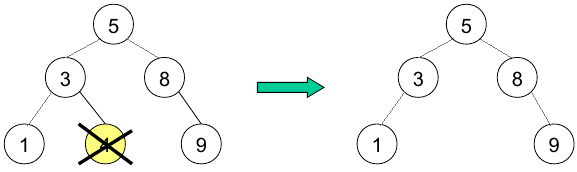
\includegraphics[width=\linewidth, scale=0.9]{tree_delete_1.png}
\captionof{figure}{Il nodo $z$ non ha sottoalberi}
\vspace{1em}
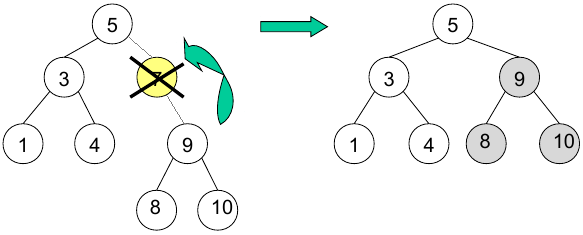
\includegraphics[width=\linewidth, scale=0.9]{tree_delete_2.png}
\captionof{figure}{Il nodo $z$ ha un sottoalbero}
\vspace{1em}
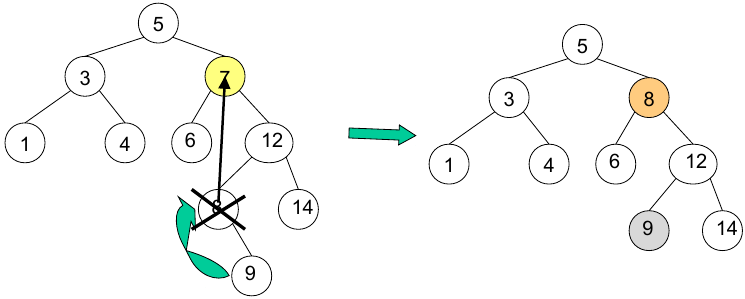
\includegraphics[width=\linewidth, scale=0.9]{tree_delete_3.png}
\captionof{figure}{Il nodo $z$ ha due sottoalberi}

\justifying

\subsection*{Complessità degli alberi binari}
Un albero si dice \emph{bilanciato} se per ogni nodo $x$ le altezze dei due sottoalberi di $x$ differiscono al massimo di 1.
$h$ è l'altezza dell'albero. 
\begin{equation*}
    h = \begin{cases}
        \varTheta(\log(n)) \quad \text{albero bilanciato}\\
        \varTheta(n)\quad \text{caso pessimo}
    \end{cases}
\end{equation*}

\begin{tabular}{l l}
    Operazione & Complessità\\
    \hline
    In-order walk & $T(n) = \varTheta(n)$ \\
    Search & $T(n) = O(h)$ \\
    Max/Min & $T(n) = O(h) $\\
    Successor & $T(n) = O(h) $\\
    Insert & $T(n) = O(h) $\\
    Delete & $T(n) = O(h) $\\
\end{tabular}
\subsection*{Alberi rosso-neri}
\begin{itemize}
    \item Sono BST abbastanza bilanciati, tali che $h = O(\log(n))$ ed è possibile realizzare tutte le operazioni più importanti in $T(n) = O(\log(n))$
    \item Un ramo non è mai più lungo del doppio di un altro
    \item Un BST è un albero RB se soddisfa le seguenti proprietà:
    \begin{enumerate}
        \item Ogni nodo è \emph{rosso} oppure \emph{nero}
        \item La radice è necessari
        \item Le foglie (\code{nil}) sono tutte nere
        \item I figli di un nodo rosso sono entrambi neri
        \item Per ogni nodo $x$ tutti i cammini da $x$ alle foglie sue discendenti contengono lo stesso numero $bh(x)$ di nodi neri. $bh(x)$ è l'\emph{altezza nera} del nodo $x$, che non viene conteggiato nella sua altezza
    \end{enumerate}
    \item Per comodità le foglie \code{nil} si usa un nodo sentinella \code{T.nil}
    \item Un albero RB con $n$ nodi interni (cioè con chiavi), ha altezza $h \le 2\log_2(n+1)$. Pertanto, \code{SEARCH}, \code{MINIMUM}, \code{MAXIMUM}, \code{SUCCESSOR}, \code{PREDECESSOR} richiedono tempo $T(n) = O(\log(n))$
    \item \code{INSERT} e \code{DELETE} sono modificate per poter rispettare le proprietà degli alberi RB, ma richiedono sempre $T(n) = O(\log(n))$
    \item Per realizzare inserimenti e cancellazioni si usa il meccanismo delle rotazioni, con \code{ROTATE-LEFT} e \code{ROTATE-RIGHT}
\end{itemize}

\centering
\vspace{1em}
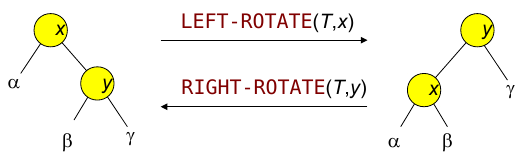
\includegraphics[width=\linewidth, scale=0.9]{rb_rotations.png}
\justifying

\subsubsection*{Inserimento}
Analogo a quello dei BST, ma per ristabilire le proprietà degli alberi RB si usa \code{RB-INSERT-FIXUP}, che viene invocato sempre su un nodo $z$ tale che \code{z.color = RED}, e al massimo $O(log(n))$ volte.

\centering
\vspace{1em}
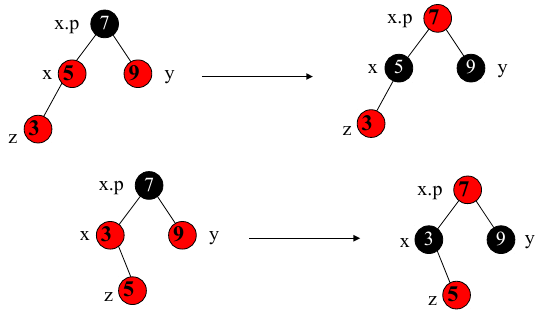
\includegraphics[width=\linewidth, scale=0.9]{rb_insert_fixup_1.png}
\captionof{figure}{$y$ rosso}
\vspace{1em}
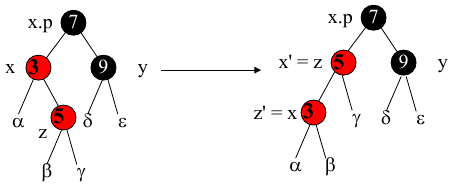
\includegraphics[width=\linewidth, scale=0.9]{rb_insert_fixup_2.png}
\captionof{figure}{$y$ nero e $z$ figlio destro di $x$}
\vspace{1em}
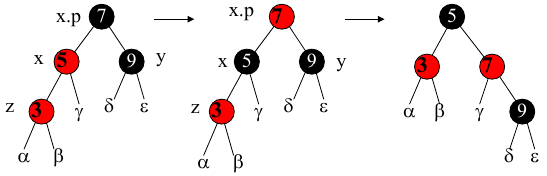
\includegraphics[width=\linewidth, scale=0.9]{rb_insert_fixup_3.png}
\captionof{figure}{$y$ nero e $z$ figlio sinistro di $x$}
\justifying

\subsubsection*{Cancellazione}
Analogo a quello dei BST. Se viene cancellato un nodo rosso non c'è bisogno di modificare i colori dei nodi, e quello che prende il suo posto è per forza nero.

\centering
\vspace{1em}
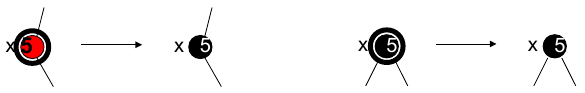
\includegraphics[width=\linewidth, scale=0.9]{rb_delete_fixup_0.png}
\captionof{figure}{$x$ rosso, oppure \`e la radice}
\vspace{1em}
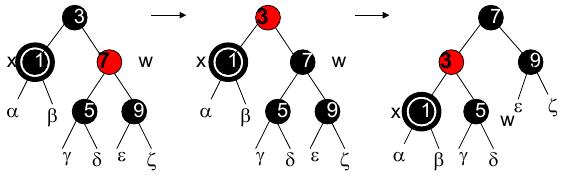
\includegraphics[width=\linewidth, scale=0.9]{rb_delete_fixup_1.png}
\captionof{figure}{$x$ nero, il fratello destro $w$ \`e rosso, e quindi il padre \`e nero}
\vspace{1em}
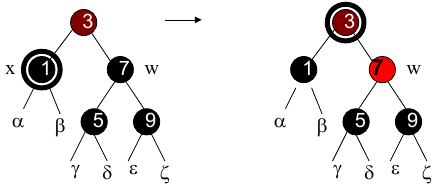
\includegraphics[width=\linewidth, scale=0.9]{rb_delete_fixup_2.png}
\captionof{figure}{$x$ nero, il fratello destro $w$ \`e nero con figli neri}
\vspace{1em}
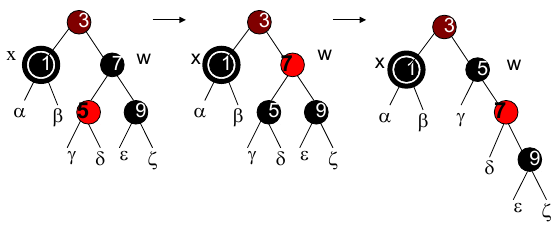
\includegraphics[width=\linewidth, scale=0.9]{rb_delete_fixup_3.png}
\captionof{figure}{$x$ nero, il fratello destro $w$ \`e nero con figlio sinistro rosso e figlio destro nero}
\vspace{1em}
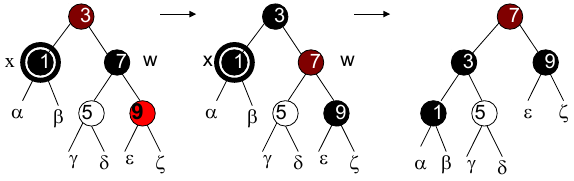
\includegraphics[width=\linewidth, scale=0.9]{rb_delete_fixup_4.png}
\captionof{figure}{$x$ nero, il fratello destro $w$ \`e nero con figlio destro rosso}
\justifying

\subsection*{Grafi}
Un grafo è una coppia $G = (V,E)$ in cui:
\begin{itemize}
    \item $V$ è un insieme di nodi detti vertici
    \item $E$ è un insieme di archi detti lati/edges. Un arco è una connessione fra due vertici, detti quindi adiacenti. Un arco è una coppia $(u,v) \in E \subseteq V^2$
    \item $|V|$ è il numero di vertici nel grafo, mentre $|E|$ è il numero di archi. Inoltre $0 \le |E| \le |V|^2$
\end{itemize}
I grafi esistono orientanti e \emph{non orientati}.
\subsubsection*{Rappresentazione in memoria}
\begin{itemize}
    \item \emph{Liste di adiacenza}: array di liste, una per nodo. Per ogni nodo, la lista contiene i nodi adiacenti ad esso. Ha complessità spaziale $S_L = \varTheta(|V|+|E|)$
    \item \emph{Matrice di adiacenza}: $m_{ij} = 1$ se c'è un arco dal nodo $i$ al nodo $j$, altrimenti è $0$. Ha complessità spaziale $S_M = \varTheta(|V|^2)$
\end{itemize}
\subsubsection*{Visita in ampiezza/Breadth-First Search}
Ha complessità $T_\text{BFS} = O(|V| + |E|)$.
\begin{itemize}
    \item Usa una politica FIFO (coda)
    \item Visito tutti i nodi a distanza 1 da $s$ (sorgente)
    \item Quando visito un nodo $u$, salvo la sua distanza da $s$ in un attributo \code{u.dist}
    \item Coloro i nodi che visito (\emph{bianco} se è da visitare, \emph{grigio} se è già stato visitato, ma bisogna completare la visita dei nodi adiacenti, \emph{nero} dopo che abbiamo visitato tutti i suoi nodi adiacenti)
    \item All'inizio tutti i nodi sono bianchi tranne $s$ che è grigio.
    \item I nodi da visitare sono in una coda (inizialmente solo $s$)
    \item A ogni iterazione, cancello dalla coda un elemento $u$ e ne visitiamo i nodi adiacenti che sono ancora bianchi (la cui distanza da $s$ sarà \code{u.dist+1})
\end{itemize}

\centering
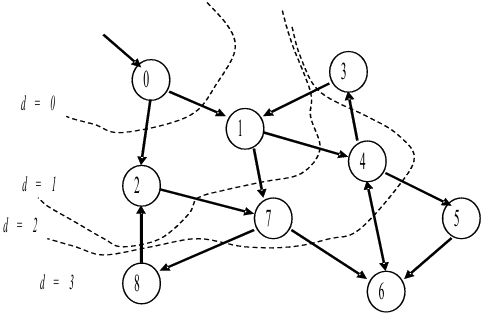
\includegraphics[width=0.7\linewidth]{graph_bfs.png}
\captionof{figure}{BFS}
\justifying

\subsubsection*{Visita in profondità/Depth-First Search}
Ha complessità $T_\text{DFS} = O(|V| + |E|)$.
\begin{itemize}
    \item Usa una politica LIFO (stack)
    \item Tiene traccia di quando un nodo è aggiunto alla pila (\code{u.d}) e di quando viene tolto (\code{u.f})
\end{itemize}

\subsubsection*{Ordinamento Topologico}
Dato un grafo orientato aciclico (DAG), un ordinamento topologico è un ordinamento lineare dei nodi del grafo tale che, se nel DAG c'è un arco $(u,v)$, allora il nodo $u$ precede $v$ nell'ordinamento (cioè che le frecce ``vanno solo in una direzione''). L'ordinamento ottenuto rispetta la precedenza tra nodi/eventi.
\begin{itemize}
    \item Visito il DAG con un algoritmo DFS
    \item quando coloro un nodo $u$ di nero, inserisco $u$ in testa alla lista
    \item Una volta visitati tutti i nodi, ottengo un ordinamento topologico 
\end{itemize}
Ha la stessa complessità di DFS, cioè $T_\text{TS} = O(|V| + |E|)$.

\subsubsection*{Cammini Minimi}
\begin{equation*}
    \delta(u,v) = \begin{cases}
        \min\left\{w(p): u\xrightarrow p v\right\} \quad \text{se $\exists$ cammino $p$ da $u$ a $v$}\\
        \infty \qquad \text{altrimenti}
    \end{cases}
\end{equation*}
\begin{itemize}
    \item $w: E \rightarrow R$ è la \emph{funzione di peso}
    \item $d[v] = \delta(s, v)$ è detto \emph{stima di cammino minimo} dalla sorgente $s$ a $v$ 
    \begin{itemize}
        \item All'inizio vale $d[v] = \infty$
        \item viene ridotto col procedere dell'algoritmo, ma $d[v] \le \delta(s, v)$
    \end{itemize}
    \item $P_i[v]$ è il \emph{predecessore di $v$} nel cammino minimo da $s$, se non esiste è \code{nil}
\end{itemize}

\subsubsection*{Rilassamento di un lato}
\begin{itemize}
    \item se $d[v] > d[u]+w(u,v)$ allora $d[v] = d[u] + w(u,v)$ e $P_i[v]=u$
\end{itemize}
\subsection*{Bellman-Ford}
\begin{itemize}
    \item Rilasso un passo alla volta partendo da s
    \item Ad ogni passo avanzo nei cammini
    \item Al $|V| - 1$-esimo passo sicuramente avrò toccato tutti i nodi raggiungibili
    \item \emph{non} converge se ci sono cicli negativi
\end{itemize}
\begin{lstlisting}
BELLMAN-FORD(adj, s)
    V = vector of nodes of adj
    allocate vectors d, Pi of size adj

    for i = 0 to |adj| - 1
        d[i] = $\infty$
    d[s] = 0
        repeat for |V| - 1 times
            for u in V
                for v in adj[u]
                    RELAX(u, v, adj, d, Pi)
    return [d, Pi]
\end{lstlisting}
\end{multicols*}
\pagebreak
\begin{multicols*}{2}
\subsection*{In Order Tree Walk}
\begin{lstlisting}
INORDER-TREE-WALK(x)
    if x != nil
        INORDER-TREE-WALK(x.left)
        print x.key
        INORDER-TREE-WALK(x.right)
\end{lstlisting}
\subsection*{Tree Search}
\begin{lstlisting}
TREE-SEARCH(x, k)
    if x == nil or k == x.key
        return x
    if k < x.key
        return TREE-SEARCH(x.left, k)
    else
        return TREE-SEARCH(x.right, k)
\end{lstlisting}
\subsection*{Tree Minimum}
\begin{lstlisting}
TREE-MINIMUM(x)
    while x.left != nil
        x = x.left
    return x
\end{lstlisting}
\subsection*{Tree Maximum}
\begin{lstlisting}
TREE-MAXIMUM(x)
    while x.right != nil
        x = x.right
    return x
\end{lstlisting}
\subsection*{Tree Successor}
\begin{lstlisting}
TREE-SUCCESSOR(x)
    if x.right != nil
        return TREE-MINIMUM(x.right)
    y = x.p
    while y != nil and x = y.right
        x = y
        y = y.p
    return y
\end{lstlisting}
\subsection*{Tree Insert}
\begin{lstlisting}
TREE-INSERT(T, z)
    y = nil
    x = T.root
    while x != nil
        y = x
        if z.key < x.key
            x = x.left
        else x = x.right
    z.p = y
    if y == nil
        T.root = z
    else if z.key < y.key
        y.left = z
    else
        y.right = z
\end{lstlisting}
\subsection*{Tree Delete}
$y$ e' il nodo da eliminare, $x$ e' quello con cui lo sostituiamo
\begin{lstlisting}
TREE-DELETE(T, z)
    if z.left == nil or z.right == nil
        y = z
    else
        y = TREE-SUCCESSOR(z)
    if y.left != nil
        x = y.left
    else
        x = y.right
    if x != nil
        T.root = x
    else if y == y.p.left
        y.p.left = x
    else
        y.p.right = x
    if y != z
        z.key = y.key
    return y
\end{lstlisting}
\subsection*{Rotazione a sinistra}
\begin{lstlisting}
ROTATE-LEFT(T, z)
    y = x.right
    x.right = y.left

    if y.left != T.nil
        y.left.p = x
    y.p = x.p
    if x.p == T.nil
        T.root = y
    else if x == x.p.left
        x.p.left = y
    else
        x.p.right = y
    y.left = x
    x.p = y
\end{lstlisting}
\subsection*{RB Tree Insert}
\begin{lstlisting}
RB-TREE-INSERT(T, z)
    y = T.nil
    x = T.root
    while x != T.nil
        y = x
        if z.key < x.key
            x = x.left
        else x = x.right
    z.p = y
    if y == T.nil
        T.root = z
    else if z.key < y.key
        y.left = z
    else
        y.right = z
    z.left = T.nil
    z.right = T.nil
    z.color = RED
    RB-INSERT-FIXUP(T, z)
\end{lstlisting}

\subsection*{RB Insert Fixup}
\begin{lstlisting}
    RB-INSERT-FIXUP(T, z)
    if z == T.root
        T.root.color = BLACK
    else 
        x = z.p
    if x.color == RED
        if x == x.p.left
            y = x.p.right
            if y.color == RED
                x.color = BLACK
                y.color = BLACK
                x.p.color = RED
                RB-INSERT-FIXUP(T, x.p)
            else if z == x.right
                z = x
                LEFT-ROTATE(T, z)
                x = z.p
            x.color = BLACK
            x.p.color = RED
            RIGHT-ROTATE(T, x.p)
        else //... 
    (come il contenuto dell'if
    associato, scabio left e right)
\end{lstlisting}
\subsection*{RB Delete}
\begin{lstlisting}
RB-DELETE(T, z)
    if z.left == T.nil 
    or z.right == T.nil
        y = z
    else
        y = TREE-SUCCESSOR(z)
    if y.left != T.nil
        x = y.left
    else 
        x = y.right
    x.p = y.p
    if y.p == T.nil
        T.root = x
    else if y = y.p.left
        y.p.left = x
    else
        y.p.right = x
    if y != z
        z.key = y.key
    if y.color = BLACK
        RB-DELETE-FIXUP(T,x)
    return y
\end{lstlisting}
\subsection*{RB Delete Fixup}
\begin{lstlisting}
RB-DELETE-FIXUP(T, x)
    if x.color == RED
    or x.p == T.nil
        x.color = BLACK
    else if x == x.p.right
        w = x.p.right
        if w.color == RED
            w.color = BLACK
            x.p.color = RED
            LEFT-ROTATE(T, x.p)
            w = x.p.right
        if w.left.color == BLACK
        and w.right.color == BLACK
            w.color = RED
            RB-DELETE-FIXUP(T, x.p)
        else if w.right.color == BLACK
            w.left.color = BLACK
            w.color = RED
            ROTATE-RIGHT(T, w)
            w = x.p.right
        w.color = x.p.color
        x.p.color = BLACK
        ROTATE-LEFT(T, x.p)
    else 
    // come le righe 4-21, scambio
    // "left" $\leftrightarrow$ "right"
\end{lstlisting}
\subsection*{Breadth First Search}
\begin{lstlisting}
BFS(G, s)
    for each u $\in G.V - \left\{s\right\}$
        u.color = WHITE
        u.dist = $\infty$
    s.color = GREY
    s.dist = 0
    Q = nil
    ENQUEUE(Q, s)
    while Q != nil
        u = DEQUEUE(Q)
        for each v $\in$ u.Adj
            if v.color == WHITE
                v.color = GREY
                v.dist = u.dist + 1
                ENQUEUE(Q, v)
    u.color = BLACK
\end{lstlisting}
\subsection*{Depth First Search}
\begin{lstlisting}
DFS(G)
    for each u $\in G.V$
        u.color = WHITE
    time = 0
    for each u $\in G.V$
        if u.color = WHITE
            DFS-VISIT(u)

DFS-VISIT(u)
    u.color = GREY
    time = time + 1
    u.d = time
    for each v $\in$ u.Adj
        if v.color = WHITE
            DFS-VISIT(v)
    u.color = BLACK
    u.f = time = time + 1
\end{lstlisting}
\subsection*{Ordinamento Topologico}
\begin{lstlisting}
TOPOLOGICAL-SORT(G)
    L = nil
    for each u $\in$ G.V
        u.color = WHITE
    for each u $\in$ G.V
        if u.color = WHITE
            TOPSORT-VISIT(L, u)
return L

TOPSORT-VISIT(L, u)
    u.color = GREY
    for each v $\in$ u.Adj
        if v.color = WHITE
            TOPSORT-VISIT(L, v)
    ... // crea l'elemento di lista x
    x.key = u
    LIST-INSERT(L, x)
    u.color = BLACK
\end{lstlisting}
\end{multicols*}

\end{document}